\documentclass[twocolumn,nofootinbib]{revtex4-1}
\usepackage{graphics}
\usepackage[caption=false]{subfig}
\usepackage{amsmath}
\usepackage{hyperref}
\usepackage{amssymb}
\usepackage{color}
\usepackage{epsfig}
\usepackage{latexsym}
\usepackage{tensor}
%\usepackage{wasysym}
\usepackage{comment}
%\usepackage{graphicx}
%\usepackage{psfrag}


%\newcommand{\gw}{gravitational wave }
%\newcommand{\gws}{gravitational waves }
\newcommand{\subgw}{_{\textrm{\scriptsize{GW}}}}
\newcommand{\ee}[1]{\!\times\!10^{#1}}
\newcommand{\prob}{{\rm Pr}}
\newcommand{\grbrate}{{{\mathcal R}_{\mathrm{grb}}}}
\newcommand{\cbcrate}{{{\mathcal R}}}
\newcommand{\diff}{{\mathrm d}}
\newcommand{\rhostar}{{\rho^*}}

\def\imbh#1{intermediate mass black hole#1(IMBH#1)\gdef\imbh{IMBH}}
\def\smbh#1{supermassive black hole#1(SMBH#1)\gdef\smbh{SMBH}}
\def\bbh#1{binary black hole#1 (BBH#1)\gdef\bbh{BBH}}
\def\bh#1{black hole#1 (BH#1)\gdef\bh{BH}}
\def\ns#1{neutron star#1 (NS#1)\gdef\ns{NS}}
\def\gw#1{gravitational wave#1 (GW#1)\gdef\gw{GW}}
\def\sn#1{core-collapse supernova#1 (CCSN#1)\gdef\sn{CCSN}}
\def\pnw#1{post-Newtonian#1 (PN#1)\gdef\pnw{PN}}
\def\eos#1{equation of state#1 (EOS#1)\gdef\eos{EOS}}
\def\grb#1{gamma-ray burst#1 (GRB#1)\gdef\grb{GRB}}
\def\amr#1{adaptive mesh refinement#1 (AMR#1)\gdef\amr{AMR}}
\def\isco#1{innermost stable circular orbit#1 (ISCO#1)\gdef\isco{ISCO}}
\def\cwb#1{Coherent WaveBurst#1 (CWB#1)\gdef\cwb{CWB}}

\newcommand{\red}[1]{{\color{red}{#1}}}
\newcommand{\about}[1]{{\color{blue}{[THIS SECTION: #1]}}}
\newcommand{\add}[1]{{\color{magenta}{[TO INCLUDE: #1]}}}
\newcommand{\JC}[1]{{\color{magenta}{[[JC #1]]}}}
\newcommand{\placeholder}[2]{{\color{red}{[PLACEHOLDER](#1):}}{\color{red}{[}}#2{\color{red}{]}}}
\providecommand{\todo}[1]{{\color{red}$\blacksquare$~\textsf{[TODO: #1]}}}


%%%%%% Useful for draft editing
\usepackage{soul} 
\usepackage{ulem} \normalem 
\newcommand{\ec}[1]{{\noindent\color{red}{\it [[#1]] }}}
\newcommand{\laura}[1]{{\color{blue}{#1}}}
\newcommand{\LC}[1]{{\color{red}{[[LC #1]]}}}
\newcommand{\AB}[1]{{\color{blue}{[[AB #1]]}}}
\newcommand{\highlight}[1]{\colorbox{yellow}{#1}}
\newcommand{\simgt}{\mbox{$^{>}_{\sim}$}}

\begin{document}

\title{Constraints On Short, Hard Gamma-Ray Burst Beaming Angles From
Gravitational Wave Observations}
\author{James Clark, Ik Siong Heng, Martin Hendry}
\date{\today}

\begin{abstract}
\dots
\end{abstract}

\maketitle

\section{Introduction}

It is common in the literature to draw inferences on the rate of binary
coalescence $\cbcrate$, given some estimate for the beaming angle $\theta$ and
the observed rate of sGRBs $\grbrate$.  In this work, we investigate what
statements can \emph{currently} be made on the beaming angle itself using the
upper limits placed on $\cbcrate$ from all-sky, all-time \gw{} searches and
explore the potential for direct inference of sGRB  beaming angles in the
advanced detector era.

\section{Inferring The sGRB Beaming Angle From Rate Measurements}
Assuming that at least some fraction of sGRBs are due to compact binary
coalescence, the observed rate of sGRBs may be written,
%
\begin{equation}\label{eq:rate2angle}
\grbrate=\epsilon\cbcrate(1-\cos \theta),
\end{equation}
%
where $\cbcrate$ is the rate of binary coalescence, $\theta$ is the beaming
angle of the outflow from the GRB and $\epsilon$ is the (generally unknown)
probability that a binary coalescence results in an observed sGRB.  In this
work, we assume
$\grbrate=10$\,Gpc$^{-3}$\,yr$^{-1}$~\cite{nakar-2007,Dietz11}.
 
Inferences of the GRB beaming angle are made from the posterior probability
density on the beaming angle $p(\theta|D,I)$.  Our goal then, is to transform
the measured posterior probability density on the rate $\cbcrate$ to a posterior
on the beaming angle.
%
First, note that the PDF $p(\theta|D,I)$ may be written as a marginalisation
over $\epsilon$ in the the joint PDF $p(\theta, \epsilon|D,I)$:
%
\begin{equation}
p(\theta) = \int_{\epsilon} p(\theta,\epsilon)~\diff \epsilon,
\end{equation}
%
where we have dropped the conditioning statements temporarily for notational
convenience.  Next, we note that the joint probability $p(\theta,\cbcrate)$ can
be written in terms of $\epsilon$ and $\cbcrate$ according to,
%
\begin{equation}
p(\theta,\epsilon) = p(\cbcrate,\epsilon)
\left\lvert\left\lvert
\frac{\partial(\cbcrate,\epsilon)}{\partial(\theta,\epsilon)}
\right\rvert\right\rvert,
\end{equation}
%
where the Jacobian matrix is given by,
% Increase matrix line spacing
\begingroup
\renewcommand*{\arraystretch}{1.5}

% matrix:
\begin{equation}
\frac{\partial (\cbcrate,\epsilon)}{\partial(\theta,\epsilon)} =
\begin{bmatrix}
\frac{\partial \cbcrate}{\partial \theta} & \frac{\partial \cbcrate}{\partial \epsilon} \\
\frac{\partial \epsilon}{\partial \theta} & \frac{\partial \epsilon}{\partial \epsilon}
\end{bmatrix}.
\end{equation}

% end line spacing increase
\endgroup
%%
Bringing all of these terms together then, and writing out the Jacobian matrix
determinant, we have
%
\begin{equation}\label{eq:marginaltheta}
p(\theta) = \frac{2\grbrate \sin
\theta~p(\cbcrate)}{(\cos\theta-1)^2}\int_{\epsilon} \frac{p(\epsilon)}{\epsilon} ~\diff
\epsilon,
\end{equation}
%
where we have assumed $\epsilon$ and $\cbcrate$ are logically independent such
that,
\begin{equation}
p(\epsilon,\cbcrate) = p(\epsilon|\cbcrate)p(\cbcrate) = p(\epsilon)p(\cbcrate).
\end{equation}
%
%
To find the target PDF $p(\theta|D,I)$ then, we require the measured coalescence
rate posterior $p(\cbcrate|D,I)$, and we must specify a prior PDF for $\epsilon$
which encapsulates assumptions made about the relative rates of compact binary
mergers and sGRBs.
 
Following~\cite{Biswas09,BradyFairhurst08}, the posterior on the binary
coalescence rate may be determined from the loudest event in the \gw{}
analysis.  Specifically, for a foreground event rate due to  binary coalescence
$\cbcrate$, the probability of obtaning no events with ranking statistic $\rho$
greater than the observed loudested event $\rhostar$ is,
%
\begin{equation}
P_F(\rhostar | \cbcrate, C_L, T) = e^{-\cbcrate C_L(\rhostar) T},
\end{equation}
%
where $C_L(\rhostar)$ is the total luminosity to which the search is sensitive
and $T$ is the duration of the search.  The overall probability of obtaining
no events with ranking statistic $\rho>\rhostar$ is the product of obtaining
no such events from foreground \emph{and} the probability of obtaining no such
events from the background in the detector, denoted $P_B(\rhostar)$,
%
\begin{equation}
P(\rhostar|\cbcrate,I) = P_B(\rhostar|I)e^{-\cbcrate C_L(\rhostar) T}
\end{equation}
%
Using a uniform prior on $\cbcrate$ and inverting the overall probability with
Bayes' theorem, we arrive at,
%
\begin{equation}\label{eq:loudestEventPosterior}
p(\cbcrate | C_L({\rhostar}), T, \Lambda) \propto p(\cbcrate) \left[ \frac{1+\Lambda
C_L(\rhostar) T}{1+\Lambda}\right] e^{-\cbcrate C_L(\rhostar) T}
\end{equation}
%
where $p(\cbcrate)$ is the prior probability distribution on the rate.  The
quantity $\hat{\Lambda}$ measures the relative probability of detecting an event
with ranking statistic $x$ due to \gw{s} versus the probability of an equally loud
event arising in the background distribution.  The reader is directed to
section\,3 of~\cite{BradyFairhurst08} for a full discussion of this quantity.


\section{Beaming Angle Limits From Past GW Searches}

In this section, we focus attention on the interpretation of rate upper limits
from past \gw{} analyses.  We first reconstruct the measured posterior on the
binary coalescence rate and go on to compute the posterior and upper limit on
the sGRB beaming angle under a range of assumptions regarding the sGRB
efficiency $\epsilon$.

The upper limit on the binary coalescence rate at confidence $\alpha$ is found
by integrating the rate posterior from zero to $\alpha$.  Assuming a uniform
prior on the rate $\cbcrate$ and using the rate posterior given by
equation~\ref{eq:loudestEventPosterior}, the upper limit on the rate
$\cbcrate_{\alpha}$ is given by equation 21 in~\cite{BradyFairhurst08}:
%
\begin{equation}
1-\alpha =  e^{-\cbcrate_{\alpha} C_L(\rhostar)T)}
\left[ 
1+ \left(\frac{\Lambda}{1+\Lambda}\right) \cbcrate_{\alpha} T C_L(\rhostar)
\right ].
\label{eq:rateIntegral}
\end{equation}
%
In the event that no \gw{} signal has been observed and the loudest event is
umabiguously due to background noise fluctuations, we are in the limit in which
$\Lambda \rightarrow 0$.  In this case, we simply have,
\begin{equation}
C_L(\rhostar)T = -\frac{\log(1-\alpha)}{\cbcrate_{\alpha}},
\end{equation}
%
and the value of $\cbcrate$ can be taken straight from the literature\footnote{Note
that this procedure necessarily confines our jet angle inferences based on
progenitor systems for which the rate upper limits are available.  Given that
the binary coalesence rate limits are quoted for canonical binary neutron star
and neutron star-black hole systems, both plausible sGRB progenitors, this
simply means our inferences on the jet angle are specific to each system and
treated separately.}

Using the most stringent 90\% confidence upper limit from \gw{} observations on
the rate of binary neutron star coalescences to date, $\cbcrate^{90\%}_{{\rm
bns}} = 1.3\times 10^{-4}$\,Mpc$^{-3}$yr$^{-1}$~\cite{S6lowmass}, gives
$C_L(\rhostar)T=17712$.  Similarly, for NS-BH systems,  $\cbcrate^{90\%}_{{\rm
nsbh}} = 3.1\times 10^{-5}$\,Mpc$^{-3}$yr$^{-1}$ gives $C_L(\rhostar)T=74277$.
The posteriors on the rates, assuming these values and $\Lambda=0$, are shown in
figure~\ref{fig:reconstructedRatePosterior}.  

\begin{figure}
\includegraphics{iLIGO/rate_posterior_s6UL_TEST_deltaEffPrior-1.0.eps}
\caption{Rate posterior for S6/VSR2,3 Low-mass Search For Compact Binary
Coalescence.\label{fig:reconstructedRatePosterior}}
\end{figure}

Figure~\ref{fig:jetPosterior} shows the posteriors on the GRB
beaming angle, using the transformation in equation~\ref{eq:rate2angleProb} and
a variety of different priors for the GRB efficiency, $\epsilon$.  The prior
pdfs are summarized in figure~\ref{fig:efficiency_priors}.
%
Finally, the quantity of interest is the upper limit on the jet
angle~$\theta^{90\%}$:
%
\begin{equation}
0.9 = \int_{\theta^{90\%}}^{\infty}p(\theta | \cbcrate^{90\%})~\diff \theta
\end{equation}
%
This is indicated with the vertical red line in figure~\ref{fig:jetPosterior}.
\textcolor{red}{TODO: combine jet posteriors onto a single plot and make a
figure showing the efficiency priors}.

\begin{figure}
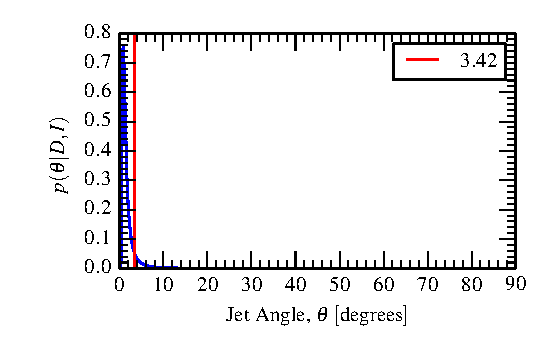
\includegraphics{iLIGO/jet_angle_posterior_s6UL_TEST_deltaEffPrior-1.0.eps}
\caption{Jet angle posterior derived from S6/VSR2,3 Low-mass Search For Compact Binary
Coalescence posterior / upper limit on compact binary coalescence
rate, assuming \emph{all} BNS result in sGRBs.\label{fig:jetPosterior}}
\end{figure}

\begin{figure}[h!]
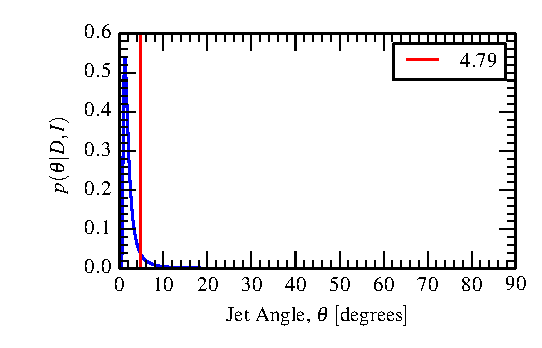
\includegraphics{iLIGO/jet_angle_posterior_s6UL_TEST_deltaEffPrior-0.5.eps}
\caption{$p(\epsilon|I)=\delta(\epsilon-0.5)$: efficiency assumed known:
$\epsilon=0.5$}
\end{figure}

\begin{figure}[h!]
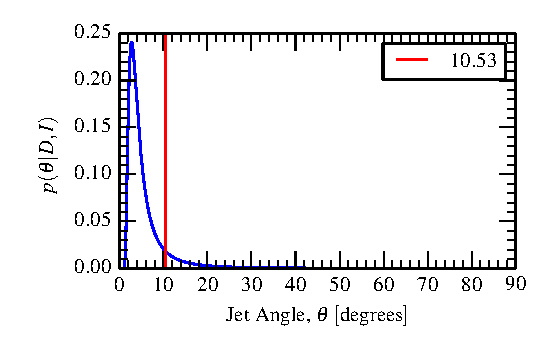
\includegraphics{iLIGO/jet_angle_posterior_s6UL_TEST_deltaEffPrior-0.1.eps}
\caption{$p(\epsilon|I)=\delta(\epsilon-0.1)$: efficiency assumed known:
$\epsilon=0.1$}
\end{figure}

\begin{figure}[h!]
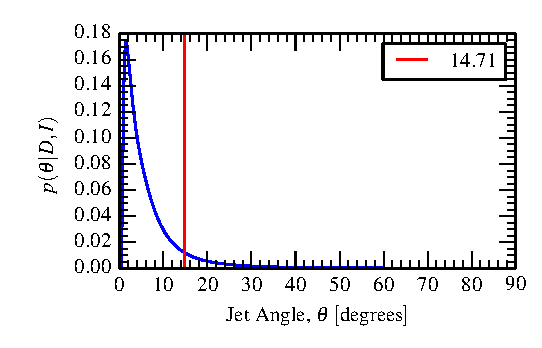
\includegraphics{iLIGO/jet_angle_posterior_s6UL_TEST_flatEffPrior-0.01-1.eps}
\caption{$p(\epsilon|I) \propto 1,~\epsilon \in (0,1]$. 
Here, we assume the GRB efficiency is $\epsilon \in (0,1]$, with no
preference where: the linearly uniform prior.  The reason for choosing a
non-zero lower bound is that the Jacobian determinant goes to $\inf$ as
$\epsilon \rightarrow 0$.  \textcolor{red}{James: I'm very open to suggestions
here as it's not clear to me that this is expected.  In practice, $\epsilon \in
[0.01,1]$}.}
\end{figure}

\begin{figure}[h!]
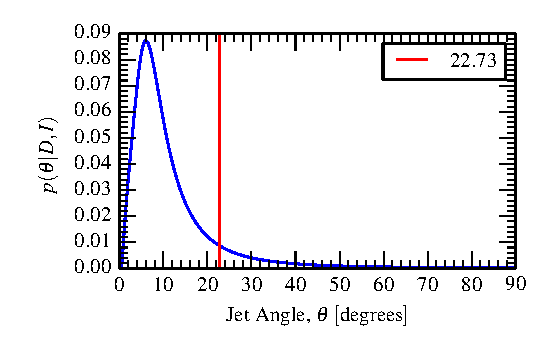
\includegraphics{iLIGO/jet_angle_posterior_s6UL_TEST_logEffPrior-0.01-1.eps}
\caption{$p(\epsilon|I) \propto 1/\epsilon,~\epsilon \in (0,1]$
Now assume the GRB efficiency is $\epsilon \in (0,1]$, with a log-uniform
prior (commonly but incorrectly referred to as the Jeffrey's prior).  Here, the
requirement of a non-zero lower bound is imposed by the normalisation for this
prior.
}
\end{figure}

\begin{figure}[h!]
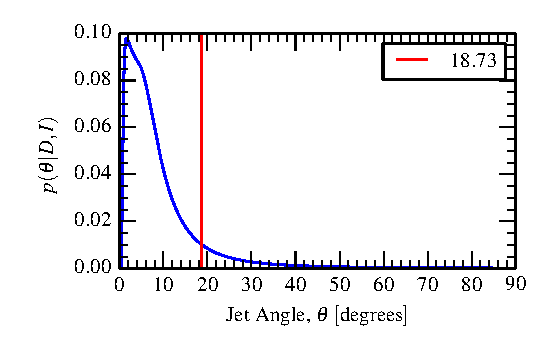
\includegraphics{iLIGO/jet_angle_posterior_s6UL_TEST_bernoEffPrior.eps}
\caption{$p(\epsilon|I) = \beta(1/2,1/2),~\epsilon \in (0,1)$.  Here, we use a
Beta distribution with shape and scale parameters of 1/2.  That prior has a
slightly surprising shape with a minimum at $\epsilon=0.5$ and shoots off to
$\infty$ as $\epsilon\rightarrow 0,1$.  It seems \emph{this} is, in fact, the
Jeffrey's prior for a Bernoulli trial (if we say a toin coss = BNS
$\rightarrow$GRB). See
\href{http://en.wikipedia.org/wiki/Jeffreys_prior}{http://en.wikipedia.org/wiki/Jeffreys\_prior}
}
\end{figure}

\begin{figure}[h!]
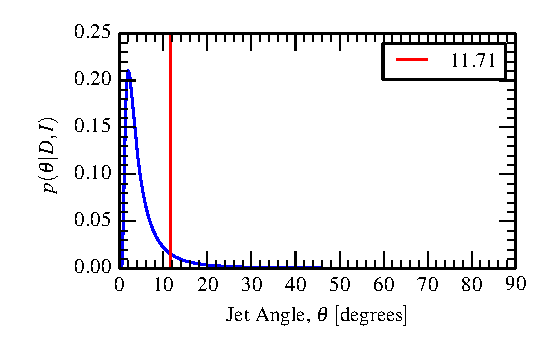
\includegraphics{iLIGO/jet_angle_posterior_s6UL_TEST_betaEffPrior-2-5.eps}
\caption{$p(\epsilon|I) = \beta(2,5),~\epsilon \in (0,1)$.  The GRB efficiency
prior is, this time, a $\beta$ distribution with shape and scale parameters 2
and 5, respectively.  This is now completely ad hoc but yields a maximum (in the
prior) around $\epsilon=0.2$ and goes to 0 as $\epsilon \rightarrow 0,1$.  So
it's a nice example of an asymmetric distribution with quite sensible (and
presumably tuneable) behaviour.}
\end{figure}

\begin{figure}[h!]
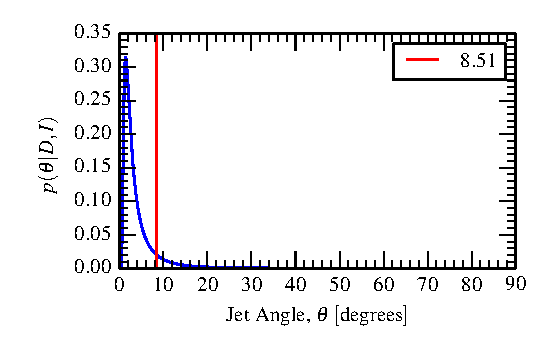
\includegraphics{iLIGO/jet_angle_posterior_s6UL_TEST_betaEffPrior-2-2.eps}
\caption{$p(\epsilon|I) = \beta(2,2),~\epsilon \in (0,1)$.  Finally, we have for
the GRB efficiency prior a $\beta$ distribution with shape and scale parameters 2
and 2, respectively.  Again, this is ad hoc but symmetric about $\epsilon=0.5$
with a cosine-like shape.}
\end{figure}

\section{Beaming Angle Inferences In The Detection Era}
In this section, we discuss an approach to measuring the GRB beaming angle based
on the binary coalescence rate as measured from a pair of detection scenarios.
In the first instance, we consider an imagined `early' science run with the the
advanced LIGO detectors where ${\mathcal O}(1)$ gravitational wave events from
binary neutron star coalescence are detected.  In the second secnario, we
consider the measurements possible with multiple gravitational wave detections.

%\subsection{For discussion: Post-detection Coalescence Rate Posterior}
%Here, we determine the formalism for the construction of a rate
%posterior in the event of single or multiple gravitational wave detections.
%%
%There needs to be no specific discussion of GRBs here, it's more general than
%that.  In fact, it's worth remembering \emph{nothing} in this paper / analysis
%(so far) has assumed contemporaneous GRB-GW detections!\footnote{although that
%does seem like a potential avenue for measuring the CBC-sGRB efficiency \dots}.
%All we actually do is assume we have independent measurements of BNS and sGRB
%rates.
%
%\textcolor{red}{Rather, the point of this discussion is to determine/describe
%a simple, natural way to construct the posterior on the rate $\cbcrate$, given
%multiple GW detections}, as expected in the advanced detector era.
%
%Recall the rate posterior from Fairhurst \& Brady~\cite{BradyFairhurst08}:
%\begin{equation}\label{eq:full_ratePosterior}
%p(\cbcrate|\rho_m, T, B) \propto p(R) \left[ \frac{1+\Lambda R
%C_L(\rho_m)T}{1+\Lambda} e^{-RC_L(\rho_m)T}\right]
%\end{equation}
%%
%Equation~\ref{eq:full_ratePosterior} is the posterior on the rate, as measured
%by the single loudest event in the search conducted.  In the equation above,
%$\Lambda$ is the likelihood of the \emph{loudest event} being from GW vs
%background and $C_L$ is the cumulative luminosity the search which produced
%loudest event $\rho_m$ is sensitive to.  It's a neat, sensible approach to
%estimating event rates given very rare measurements.  That is, it seems like a
%Good Thing / natural for constructing a rate posterior where we only expect a
%single signal trigger from a population of potentially trigger-inducing events.
%It also seems sensible:
%%
%\begin{itemize}
%\item in the absence of convincing detections (loudest event is unlikely to be a
%signal; $\Lambda \rightarrow 0$),
%\item for a single, convincing detection (loudest event is very likely to be a
%signal; $\Lambda \rightarrow \infty$).
%\end{itemize}
%%
%It's worth highlighting here that there is absolutely nothing \emph{preventing}
%one from using the loudest event statistic when we expect more than one signal
%trigger; regardless of how many events we have, there's always going be a
%loudest one and we can always determine the probability of obtaining a trigger
%that loud, given the sensitivity of the search and a population model.  Indeed,
%consider the key components in the ocnstruction of the L.E. posterior:
%%
%\begin{enumerate}
%\item The loudest event, characterised by, say, single IFO signal-to-noise ratio
%$\rho$.  Label this loudest value $\rho_m$.
%\item The probability of obtaining zero events with $\rho>\rho_m$ from a
%population of signals; this is formed from knowledge of the sensitivity of the
%analysis and a population model.  It does not require that there be only a
%single signal observed in the experiment.
%\item The probability of obtaining zero events with $\rho>\rho_m$, from a
%population of background fluctuations (Gaussian or otherwise).
%\end{enumerate}
%%
%The (potential) issue at hand is the following: suppose the most
%optimistic rate estimates are correct and aLIGO instantaneously reaches full
%design sensitivity.  In one year, we will have acquired ${\mathcal O}(100)$ BNS
%detections.  That's an entire year of measurements and a sizeable population of
%SNR measurements.  Here's the big question: 
%\begin{quote}
%{\bf \textcolor{red}{If we form the rate
%posterior from the loudest event, are we in any sense `throwing away'
%information by considering only the loudest trigger?}}
%\end{quote}
%Equally importantly (and, at the risk of sounding glib, not necessarily the same
%point\dots):
%\begin{quote}
%{\bf \textcolor{red}{Does the L.E. formalism reflect what we'll actually do
%with, say, 100 BNS detections in aLIGO?}}
%\end{quote}
%
%Without thinking about it too hard, it `feels' like we're literally throwing
%away 99\% of the information gathered in the experiment.  But is that true?
%That is, if we use the observation time of the experiment together with an
%estimate of the distance / volume sensitivity of the search, is there actually
%any more information to be gleaned from a sample of GW triggers than is already
%present in the value of the loudest trigger?  Is it perhaps the case that the
%loudest event probes the \emph{tail} of the SNR distribution, while a sample
%of triggers allows one to better estimate the full distribution of SNRs?

%\subsection{Alternative Rate Posterior Construction From \S 14 in Gregory}
\subsection{Inferring The Detection Rate}
Gregory's book, `Logical Data Analysis For The Physical Sciences' has an entire
chapter (\S 14) devoted to `Bayesian Inference With Poisson Sampling'.  This
seems to match our problem rather well.  In particular, he derives expressions
for a Poisson rate posterior in \S 14.3, `Signal + known background' and \S
14.4, `Analysis of ON/OFF measurements' (``we want to infer the source rate, s,
when the background rate, b, is imprecisely measured'').


\subsubsection{Known Background Rate}
It's tempting to jump straight into the On/off measurement stuff in \S~14.4 of
Gregory, where the construction of the rate posterior includes the raw
measurements of background rate.  I actually think this over-complicates things;
if we wanted to do follow that procedure, we have to figure out the expected FAR
for a given size of template bank etc.  There's a pretty well-established
procedure for measuring this number: time-slides.  In fact, we don't even have
to do any analysis.  Figure 3 (left panel) from the observing scenarios paper
tells us everything we need to know.  Specifically, the following sentance has
the information we need:
\begin{quote}
``We conservatively estimate a $\rho_c$ threshold of 12 is required for a false rate below
$\sim 10^{−2}$\,yr$^{−1}$.''
\end{quote}
%
So let $b=10^{-2}$\,yr$^{-1}$.  From there, we can get the detection rate
posterior using equations 14.10--14.12 of Gregory.  The measured rate $r$
consists of two components, one due to a signal of interest, $s$, and the other
a known background rate, $b$:
\begin{equation}
r = s + b
\begin{cases}
s = \text{signal rate} \\
b = \text{background rate}
\end{cases}
\end{equation}
%
Since the background rate is known,
\begin{equation}
p(s|n,b,I) = p(r|n,b,I),
\end{equation}
%
where $n$ is the number of \gw{} detections.  From eq 14.8 of Gregory, we get
to:
\begin{equation}
p(s|n,b,I) = C \frac{ T\left[(s+b)T\right]^n e^{-(s+b)T}}{n!},
\end{equation}
%
where,
\begin{eqnarray}
C^{-1} & = &\frac{e^{-bT}}{n!} \int_0^{\infty}\diff(sT)(s+b)^n T^n e^{-sT}\\
& = & \sum_{i=0}^n \frac{ (bT)^i e^{-bT}}{i!}.
\end{eqnarray}
%
So, in this approach we only need three pieces of information which constitute
the observing scenario:
\begin{enumerate}
\item $n$, the number of triggers.  This should be \emph{all} triggers:
background plus signal.  Note, however, that the operating point of the search
is such that the number of background triggers can reasonably be expected to be
$\ll 1$.
\item $T$, the observation time / science run duration.  To be taken directly
from the scenarios paper.
\item $b$, the background rate.  As discussed, this is known from many previous
studies and, again, is a number we can take directly from the observing
scenarios document.
\end{enumerate}


 
\subsubsection{Unknown Background Rate: `On/Off Measurement'}
Gregory also has a neat formalism for including a \emph{measured} background
rate.  This is very interesting and useful for general rates measurements but I
don't really think it's something we need for this paper, since the background
rate is known\footnote{Put another way: we can take the background rate directly
from the observing scenarios paper and we'll save a lot of extra work and we'll
be perfectly consistent with the Collaborations' official projections.}.  I'll
include the expressions below for now, it seems like extremely important stuff
for the rates sub-group (I believe Matt West is doing something with it).

The posterior on the rate of GW events \emph{measured in the science run} is,
\begin{equation}\label{eq:signal_rate_posterior}
p(s | N_{\textrm{on}}, I) = \sum_{i=0}^{N_{\textrm{on}}} C_i
\frac{T_{\textrm{on}} (sT_{\textrm{on}})^i e^{-s T_{\textrm{on}} }}{i!},
\end{equation}
where,
\begin{equation}
C_i \approx \frac{ \left(1 + \frac{T_{\textrm{off}}}{T_{\textrm{on}}}\right)^i
\frac{(N_{\textrm{on}} + N_{\textrm{off}} - i )!}{(N_{\textrm{on}}-i)!} }
{\sum_{j=0}^{N_{\textrm{on}}} \left(1 +
\frac{T_{\textrm{off}}}{T_{\textrm{on}}}\right)^j\frac{(N_{\textrm{on}} +
N_{\textrm{off}} - j )!}{(N_{\textrm{on}}-j)!}},
\end{equation}
%
and the quantities in both terms are as follows,
\begin{itemize}
\item $N_{\textrm{on}}$ is the number of zero-lag events observed in a science
run of duration $T_{\textrm{on}}$.
\item $N_{\textrm{off}}$ is the number of time-slide events observed in total
background time $T_{\textrm{off}}$.
\end{itemize}
%
\subsection{Inferring The Binary Coalescence Rate}
Now, I placed emphasis on $s$ being the event rate measured in the data with
good reason.  We are interested in the binary coalescence rate $\cbcrate$.  This
is not the same thing as the signal rate $s$.  However, the conversion between
signal rate and coalescence rate is precisely what the `rates'
paper~\cite{rates_paper} was all about!

In particular,  the detection rate for a given type of binary coalescence in
LIGO-Virgo is given by equation\,1 in~\cite{rates_paper},
\begin{equation}
%\dot{N} = \cbcrate \times N_G,
s = \cbcrate \times N_G,
\end{equation}
%
where $\cbcrate$ is the coalescence rate of that type of binary per galaxy and
$N_G$ is the number of galaxies accessible with a search for the relevant binary
type.  $N_G$ is well approximated at large distances by,
%
\begin{equation}
N_G = \frac{4}{3} \pi \left( \frac{D_{\textrm{horizon}}}{\textrm{Mpc}}
\right)^3 (2.26)^{-3} (0.0116).
\end{equation}
%
The reader is directed to~\cite{rates_paper} for a discussion of the numerical
factors in the equation above.

Finally, we recognise that $\dot{N}$ is the signal rate $s$ in
equation~\ref{eq:signal_rate_posterior} so that we arrive at the desired
posterior on the binary coalescence rate, 
%
\begin{eqnarray}
p(\cbcrate|N_{\textrm{det}},I) & = & p(s|N_{\textrm{det}},I) \left|\frac{\diff
s}{\diff \cbcrate}\right| \\
& = & N_G . p(s|N_{\textrm{det}},I)
\end{eqnarray}
%
If the above reasoning is sound, then `all' we require to move forward are
sensible numbers of zero-lag and background events and observation times.

\section{Summary of Gregory-Posterior Experiment}
Here's the general procedure:
\begin{enumerate}
\item Compute horizon distance from noise curve: $D_{\mathrm{horizon}}$,
assuming $\rho_c=12$ (as in rates paper).
\item Find number of galaxies accessible to this horizon distance from:
\begin{equation}
N_G = \frac{4}{3} \pi \left( \frac{D_{\textrm{horizon}}}{\textrm{Mpc}}
\right)^3 (2.26)^{-3} (0.0116).
\end{equation}
\item Detection rate is $\dot{N} = R \times N_G$, where $R$ is the binary
coalescence rate
\item Use $\dot{N}$ to determine number of GW-detections in $T_{\mathrm{obs}}$=1 year
$N_{\mathrm{det}}$
\item Compute \emph{detection} rate posterior, $p(s|N_{\textrm{on}},I)$.  The
rate posterior is then given by 
\begin{eqnarray}
p(\cbcrate|N_{\textrm{on}},I) & = & p(s|N_{\textrm{on}},I) \left|\frac{\diff
s}{\diff \cbcrate}\right| \\
& = & N_G . p(s|N_{\textrm{on}},I)
\end{eqnarray}
\end{enumerate}
%
Note, however, that steps 1-4 are already done for us in the prospects document;
the only ingredients we need are the detection rates for the observing scenarios
and the the FAR for the threshold used to get those rates.  All of this
information can be taken \emph{directly} from the observing scenarios paper.

In particular, we require the expected number of on-source events
$N_{\mathrm{on}}$ and the expected number of off-source events
$N_{\mathrm{off}}$.  We can find $N_{\mathrm{on}}$ using the search
\emph{volumes} $V_{\mathrm{search}}$ in the observing scenarios paper:
%
\begin{equation}
N_{\mathrm{det}} = \cbcrate \times V_{\mathrm{search}}
\end{equation}

We now outline the projected observing scenarios.  These are taken directly
from~\cite{ade_prospects}.  There are four scenarios in that paper,
corresponding to different run durations, epochs (i.e., sensitivity achieved)
for aLIGO/AdVirgo.  There are also three numbers in use for the binary
coalescence rate (the ``low'', ``realistic'' and ``high'' rates).  In the
interests of brevity we will consider the projected 2016--17 run (``early''
detection scenario as described here) and the fully advanced 2022+ run (``late''
in this work).  For each epoch, we will produce results for the ``realistic''
and ``high'' rates.   We can very easily include other scenarios/rates.
Table~\ref{table:scenarios} summarizes the observing scenarios.

Note that the search volume is given by,
\begin{equation}\label{eq:search_volume}
V_{\mathrm{search}} = \frac{4}{3}\pi D_{\mathrm{sens}}^3 \times \gamma T,
\end{equation}
%
where $D_{\mathrm{sens}}$ is the BNS sensemon range ($D_{\mathrm{hor}}/2.26$),
$T$ is the duration of the science run (i.e., observation time) and $\gamma$ is
the \emph{duty} cycle for the science run.  Following~\cite{ade_prospects}, we
take $\gamma=0.5$.  Since there is a range in the horizon distances to account
for uncertainty in the sensitivity of the early configuration of the detectors,
we compute use the arithmetic mean of the horizon distance when computing the
search volume.
%Finally, the expected number of detections is given by,
%\begin{equation}\label{eq:ndet}
%N_{\mathrm{det}} = \cbcrate \times \langle V_{\mathrm{search}} \rangle
%\end{equation}

\begin{table}
\centering
\begin{tabular}{l c c c c c }
\toprule
Epoch & $T$ & $D_{\mathrm{hor}}$ &
$\langle V_{\mathrm{search}}\rangle$ & $\cbcrate$ & $N_{\mathrm{det}}$ \\
 & [yr] & [Mpc] & [Mpc$^3$yr] &  [Mpc$^{-3}$yr$^{-1}$] \\
\colrule
2016--17 & 0.5 & 80--120 & $1.05\times10^6$ & $10^{-6}$ & 1.3 \\
2016--17 & 0.5 & 80--120 & $1.05\times10^6$ & $10^{-5}$ & 13 \\
2022+ & 1 & 200 & $4\times10^7$ & $10^{-6}$ & 40 \\
2022+ & 1 & 200 & $4\times10^7$ & $10^{-5}$ & 400 \\
\botrule
\end{tabular}
\caption{Advanced detector era observing scenarios considered in this work.  $T$
is the expected duration of the science run and $D_{\mathrm{hor}}$ is the BNS
horizon distance for the sensitivity expected to be acheived at the given epoch.
$\langle V_{\mathrm{search}}\rangle $ is the sensitive volume of the search,
where the angled brackets $\langle \rangle$ indicate averaging over the range
in horzizon distance, $\cbcrate$ is the assumed BNS coalescence rate and
$N_{\mathrm{det}}$ is the expected number of \gw{} detections.  Note that the
quoted search volume accounts for a network duty cycle of $\sim 50\%$.
Full details may be foud in~\cite{ade_prospects}.\label{table:scenarios}}
\end{table}



Figures to include here
\begin{itemize}
\item Rate posteriors
\item Jet posteriors for 3 delta function efficiency priors (0.1, 0.5, 1.0)
\item Jet posterior (and jet-efficiency posterior) for uniform efficiency prior
\item Jet posterior (and jet-efficiency posterior) for log-uniform efficiency
prior 
\item Jet posterior (and jet-efficiency posterior) Beta distribution with
$\beta(1/2,1/2)$ (Jeffrey's)
\item Jet posterior (and jet-efficiency posterior) Beta distribution with
$\beta(2,5)$ (Jeffrey's).
\end{itemize}

Other figures to make
\begin{itemize}
\item Plot the efficiency priors
\item iLIGO jet posterior for efficiency prior $\beta(a,b)$ with $(a,b)$ chosen
such that the maximum is at 0.5
\item jet-efficiency posteriors for iLIGO
\end{itemize}


\begin{figure}%[ht]
\centering
\subfloat[Part1][Rate Posterior (realistic)]
{\scalebox{1}{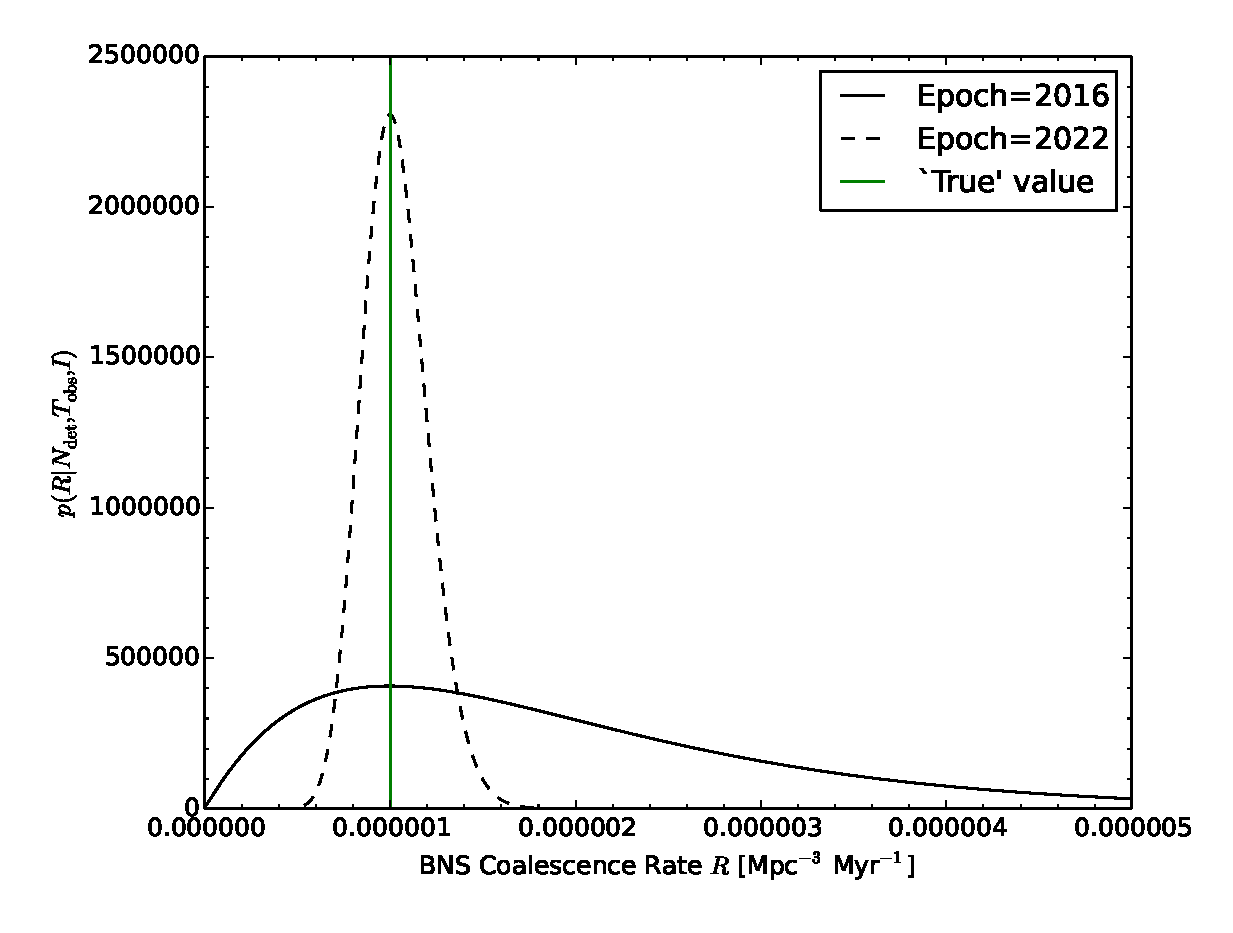
\includegraphics{aLIGO/rate_re.eps}}\label{fig:re_rate}}\\
\subfloat[Part2][Rate Posterior (high)]
{\scalebox{1}{\includegraphics{aLIGO/rate_high.eps}}\label{fig:high_rate}}
\caption{Rate Posteriors}
\end{figure}

\subsection{Validation}

\begin{figure}%[ht]
\centering
\subfloat[Part1][Jet Angle Posterior (realistic)]
{\scalebox{1}{\includegraphics{aLIGO/angle_re_delta,0.5_sim_theta-10.0_epsilon-0.5.eps}}\label{fig:jet1low}}\\
\subfloat[Part2][Jet Angle Posterior (high)]
{\scalebox{1}{\includegraphics{aLIGO/angle_high_delta,0.5_sim_theta-10.0_epsilon-0.5.eps}}\label{fig:jet1high}}\\
\caption{Jet Posteriors For $\theta_{\mathrm{true}} = 10^{\circ}$,
$\epsilon=0.5$, with prior pdf $p(\epsilon|I) = \delta(\epsilon-0.5)$.}
\end{figure}

\begin{figure}%[ht]
\centering
\subfloat[Part1][Jet Angle Posterior (realistic)]
{\scalebox{1}{\includegraphics{aLIGO/angle_re_uniform_sim_theta-10.0_epsilon-0.5.eps}}\label{fig:jet2low}}\\
\subfloat[Part2][Jet Angle Posterior (high)]
{\scalebox{1}{\includegraphics{aLIGO/angle_high_uniform_sim_theta-10.0_epsilon-0.5.eps}}\label{fig:jet2high}}\\
\caption{Jet Posteriors For $\theta_{\mathrm{true}} = 10^{\circ}$,
$\epsilon=0.5$, with prior pdf $p(\epsilon|I) = U(0.01,1)$.}
\end{figure}

\begin{figure}%[ht]
\centering
\subfloat[Part1][Jet Angle Posterior (realistic)]
{\scalebox{1}{\includegraphics{aLIGO/angle_re_jeffreys_sim_theta-10.0_epsilon-0.5.eps}}\label{fig:jet2low}}\\
\subfloat[Part2][Jet Angle Posterior (high)]
{\scalebox{1}{\includegraphics{aLIGO/angle_high_jeffreys_sim_theta-10.0_epsilon-0.5.eps}}\label{fig:jet2high}}\\
\caption{Jet Posteriors For $\theta_{\mathrm{true}} = 10^{\circ}$,
$\epsilon=0.5$, with prior pdf $p(\epsilon|I) = \beta(\frac{1}{2},\frac{1}{2}$.}
\end{figure}

\subsection{Unknown $\theta_{\mathrm{jet}}$}

\begin{figure}%[ht]
\centering
\subfloat[Part1][Jet Angle Posterior (realistic)]
{\scalebox{1}{\includegraphics{aLIGO/angle_re_delta_0p5.eps}}\label{fig:jet1low_unknown}}\\
\subfloat[Part2][Jet Angle Posterior (high)]
{\scalebox{1}{\includegraphics{aLIGO/angle_high_delta_0p5.eps}}\label{fig:jet1high_unknown}}\\
\caption{Jet Posteriors For Unknown Jet Angle, prior pdf $p(\epsilon|I) = \delta(\epsilon-0.5)$}
\end{figure}

\begin{figure}%[ht]
\centering
\subfloat[Part1][Jet Angle Posterior (realistic)]
{\scalebox{1}{\includegraphics{aLIGO/angle_re_delta_1.eps}}\label{fig:jet1low_unknown}}\\
\subfloat[Part2][Jet Angle Posterior (high)]
{\scalebox{1}{\includegraphics{aLIGO/angle_high_delta_1.eps}}\label{fig:jet1high_unknown}}\\
\caption{Jet Posteriors For Unknown Jet Angle, prior pdf $p(\epsilon|I) =
\delta(\epsilon-1.0)$}
\end{figure}

\begin{figure}%[ht]
\centering
\subfloat[Part1][Jet Angle Posterior (realistic)]
{\scalebox{1}{\includegraphics{aLIGO/angle_re_uniform_0p01-1.eps}}\label{fig:jet1low_unknown}}\\
\subfloat[Part2][Jet Angle Posterior (high)]
{\scalebox{1}{\includegraphics{aLIGO/angle_high_uniform_0p01-1.eps}}\label{fig:jet1high_unknown}}\\
\caption{Jet Posteriors Unknown Jet Angle, prior pdf $p(\epsilon|I) = U(0.01,1)$.}
\end{figure}


\begin{figure}%[ht]
\centering
\subfloat[Part1][Jet Angle Posterior (realistic)]
{\scalebox{1}{\includegraphics{aLIGO/angle_re_jeffreys.eps}}\label{fig:jet1low_unknown}}\\
\subfloat[Part2][Jet Angle Posterior (high)]
{\scalebox{1}{\includegraphics{aLIGO/angle_high_jeffreys.eps}}\label{fig:jet1high_unknown}}\\
\caption{Jet Posteriors Unknown Jet Angle, prior pdf $p(\epsilon|I) =
\beta(\frac{1}{2},\frac{1}{2})$.}
\end{figure}


\section{Conclusion}

\appendix
\section{Priors}
\begin{figure}%[ht]
\centering
%\subfloat[Part1][Jet Angle Posterior (realistic)]
{\scalebox{1}{\includegraphics{iLIGO/priors.eps}}\label{fig:priors}}\\
%\subfloat[Part2][Jet Angle Posterior (high)]
%{\scalebox{1}{\includegraphics{aLIGO/angle_high_uniform_sim_theta-10.0_epsilon-0.5.eps}}\label{fig:jet2high}}\\
\caption{Priors}
\end{figure}

\section{Jacobian Calculation}
This doesn't need to be in the publication, these are just notes for James'
benefit and possibly verification.

\begin{equation}
\cbcrate=\frac{\grbrate}{\epsilon(1-\cos \theta)},
\end{equation}

\begin{equation}
p(\theta) = \int_{\epsilon} p(\theta,\epsilon)~\diff \epsilon,
\end{equation}

\begin{equation}
p(\theta,\epsilon) = p(\cbcrate,\epsilon)
\left\lvert\left\lvert
\frac{\partial(\cbcrate,\epsilon)}{\partial(\theta,\epsilon)}
\right\rvert\right\rvert,
\end{equation}

% Increase matrix line spacing
\begingroup
\renewcommand*{\arraystretch}{1.5}

% matrix:
\begin{equation}
\frac{\partial (\cbcrate,\epsilon)}{\partial(\theta,\epsilon)} =
\begin{bmatrix}
\frac{\partial \cbcrate}{\partial \theta} & \frac{\partial \cbcrate}{\partial \epsilon} \\
\frac{\partial \epsilon}{\partial \theta} & \frac{\partial \epsilon}{\partial \epsilon}
\end{bmatrix}.
\end{equation}

% end line spacing increase
\endgroup

\begin{eqnarray}
\frac{\partial \cbcrate}{\partial \theta} & = &
-\frac{\grbrate\sin\theta}{\epsilon(\cos\theta - 1)^2}\\
\frac{\partial \cbcrate}{\partial \epsilon} & = &
\frac{\grbrate}{\epsilon^2(\cos\theta-1)}\\
\frac{\partial \epsilon}{\partial \theta} & = &
-\frac{\grbrate\sin\theta}{\cbcrate(\cos\theta-1)^2}\\
\frac{\partial \epsilon}{\partial \epsilon} & = & 1\\
\end{eqnarray}

\begin{eqnarray}
\left\lvert
\frac{\partial(\cbcrate,\epsilon)}{\partial(\theta,\epsilon)}
\right\rvert & = & \frac{\partial \cbcrate}{\partial \theta}
\frac{\partial \epsilon}{\partial \epsilon} - \frac{\partial \cbcrate}{\partial
\epsilon}\frac{\partial \epsilon}{\partial \theta} \\
& = & -\frac{2\sin\theta}{\epsilon(\cos\theta-1)^2}
\end{eqnarray}
%
Finally:
\begin{equation}
\left\lvert\left\lvert
\frac{\partial(\cbcrate,\epsilon)}{\partial(\theta,\epsilon)}
\right\rvert\right\rvert = \frac{2\grbrate\sin\theta}{\epsilon(\cos\theta-1)^2} 
\end{equation}

\section{Null-detection Jet Angle Posteriors With Different Priors}

\bibliography{grb_beams}

\end{document}
